% --------------------------------------------------------
% DEFINIÇÕES DO DOCUMENTO
% --------------------------------------------------------

\documentclass[
	% -- opções da classe memoir --
	12pt,				% tamanho da fonte
	openright,			% capítulos começam em pág ímpar (insere página vazia caso preciso)
	oneside,			% para impressão em verso e anverso. Oposto a twoside
	a4paper,			% tamanho do papel.
	% -- opções da classe abntex2 --
	%chapter=TITLE,		% títulos de capítulos convertidos em letras maiúsculas
	%section=TITLE,		% títulos de seções convertidos em letras maiúsculas
	%subsection=TITLE,	% títulos de subseções convertidos em letras maiúsculas
	%subsubsection=TITLE,% títulos de subsubseções convertidos em letras maiúsculas
	% -- opções do pacote babel --
	english,			% idioma adicional para hifenização
	french,				% idioma adicional para hifenização
	spanish,			% idioma adicional para hifenização
	brazil,				% o último idioma é o principal do documento
	]{lib/abntex2}


% --------------------------------------------------------
% PACOTES
% --------------------------------------------------------
\usepackage{cmap}				% Mapear caracteres especiais no PDF
\usepackage{lmodern}			% Usa a fonte Latin Modern
\usepackage[T1]{fontenc}		% Selecao de codigos de fonte.
\usepackage[utf8]{inputenc}		% Codificacao do documento (conversão automática dos acentos)
\usepackage{lastpage}			% Usado pela Ficha catalográfica
\usepackage{indentfirst}		% Indenta o primeiro parágrafo de cada seção.
\usepackage{color}				% Controle das cores
\usepackage{graphicx}			% Inclusão de gráficos
\usepackage{lipsum}				% para geração de dummy text

\let\printglossary\relax
\let\theglossary\relax
\let\endtheglossary\relax
\usepackage{lib/update-abntex}

\usepackage[brazilian,hyperpageref]{}	 % Paginas com as citações na bibl
\usepackage{microtype} 

\usepackage{silence}
%Disable all warnings issued by latex starting with "You have..."
\WarningFilter{latex}{You have requested package}
\usepackage[alf, abnt-etal-list=0 ]{lib/abntex2cite}	% Citações padrão ABNT
\usepackage[br]{lib/nicealgo}       % Pacote para criação de algoritmos
\usepackage{lib/customizacoes}      % Pacote de customizações do abntex2

\usepackage{listings}
\usepackage[normalem]{ulem} % Strikethrough package

% --------------------------------------------------------
% CONFIGURAÇÕES DE PACOTES
% --------------------------------------------------------

% Configurações do pacote listing
\renewcommand{\lstlistingname}{Código} %Mudança no caption do listing para Código
\renewcommand{\lstlistlistingname}{Lista de códigos} %Mudança no caption da lista de listings.


% Configurações do pacote backref
\renewcommand{\familydefault}{\sfdefault}
% Usado sem a opção hyperpageref de backref
% \renewcommand{\backrefpagesname}{Citado na(s) página(s):~}
% Texto padrão antes do número das páginas
% \renewcommand{\backref}{}
% Define os textos da citação
% \renewcommand*{\backrefalt}[4]{
% 	\ifcase #1 %
% 		Nenhuma citação no texto.%
% 	\or
% 		Citado na página #2.%
% 	\else
% 		Citado #1 vezes nas páginas #2.%
% 	\fi}%


% --------------------------------------------------------
% INFORMAÇÕES DE DADOS PARA CAPA E FOLHA DE ROSTO
% --------------------------------------------------------

\titulo{Sistema colaborativo para o rastreamento em tempo real de alertas de segurança pública}
\autor{Bruno José Papa}
\local{Bauru}
\data{Agosto/2021}
\orientador{Prof. Dr. Roberta Spolon}
\instituicao{%
  Universidade Estadual Paulista ``Júlio de Mesquita Filho''
  \par
  Faculdade de Ciências
  \par
  Sistemas de Informação}
\tipotrabalho{Trabalho de Conclusão de Curso}
\preambulo{Trabalho de Conclusão de Curso do Curso de Bacharelado em Sistemas de Informação da Universidade Estadual Paulista ``Júlio de Mesquita Filho'', Faculdade de Ciências, Campus Bauru.}


% --------------------------------------------------------
% CONFIGURAÇÕES PARA O PDF FINAL
% --------------------------------------------------------

% alterando o aspecto da cor azul
\definecolor{blue}{RGB}{41,5,195}

% informações do PDF
\makeatletter
\hypersetup{
     	%pagebackref=true,
		pdftitle={\@title},
		pdfauthor={\@author},
    	pdfsubject={\imprimirpreambulo},
	    pdfcreator={LaTeX with abnTeX2},
		pdfkeywords={abnt}{latex}{abntex}{abntex2}{trabalho acadêmico},
		colorlinks=true,       		% false: boxed links; true: colored links
    	linkcolor=blue,          	% color of internal links
    	citecolor=blue,        		% color of links to bibliography
    	filecolor=magenta,      		% color of file links
		urlcolor=blue,
		bookmarksdepth=4
}
\makeatother


% ---
% Posiciona figuras e tabelas no topo da página quando adicionadas sozinhas
% em um página em branco. Ver https://github.com/abntex/abntex2/issues/170
\makeatletter
\setlength{\@fptop}{5pt} % Set distance from top of page to first float
\makeatother
% ---

% ---
% Possibilita criação de Quadros e Lista de quadros.
% Ver https://github.com/abntex/abntex2/issues/176
%
\newcommand{\quadroname}{Quadro}
\newcommand{\listofquadrosname}{Lista de quadros}

\newfloat[chapter]{quadro}{loq}{\quadroname}
\newlistof{listofquadros}{loq}{\listofquadrosname}
\newlistentry{quadro}{loq}{0}

% configurações para atender às regras da ABNT
\setfloatadjustment{quadro}{\centering}
\counterwithout{quadro}{chapter}
\renewcommand{\cftquadroname}{\quadroname\space} 
\renewcommand*{\cftquadroaftersnum}{\hfill--\hfill}

\setfloatlocations{quadro}{hbtp}
% ---


% --------------------------------------------------------
% ESPAÇAMENTOS ENTRE LINHAS E PARÁGRAFOS
% --------------------------------------------------------

% O tamanho do parágrafo é dado por:
\setlength{\parindent}{1.3cm}

% Controle do espaçamento entre um parágrafo e outro:
\setlength{\parskip}{0.2cm}


% --------------------------------------------------------
% COMPILANDO O ÍNDICE
% ---------------------------------------------------
\makeindex
% ---
 
% ---
% GLOSSARIO
% ---
\makeglossaries
% ---
% Exemplo de configurações do glossairo
\renewcommand*{\glsseeformat}[3][\seename]{\textit{#1}  
 \glsseelist{#2}}
% ---
 
% --------------------------------------------------------
% INÍCIO DO DOCUMENTO
% --------------------------------------------------------

\begin{document}

% Seleciona o idioma do documento (conforme pacotes do babel)
\selectlanguage{brazil}

% Retira espaço extra obsoleto entre as frases.
\frenchspacing


% --------------------------------------------------------
% ELEMENTOS PRÉ-TEXTUAIS
% --------------------------------------------------------

% Capa
\imprimircapa

% Folha de rosto
% (o * indica que haverá a ficha bibliográfica)
\imprimirfolhaderosto*

% TODO: Inserir a ficha bibliografica
% \begin{fichacatalografica}
% 	\sffamily
% 	\vspace*{\fill}					% Posição vertical
% 	\begin{center}					% Minipage Centralizado
% 		\fbox{\begin{minipage}[c][7.5cm]{12.5cm}		% Largura
% 			\small
% 			\imprimirautor
% 			\hspace{0.5cm} \imprimirtitulo  / \imprimirautor. --
% 			\imprimirlocal, \imprimirdata-
% 			\hspace{0.5cm} \pageref{LastPage} p. : il. (algumas color.) ; 30 cm.\\
% 			\hspace{0.5cm} \imprimirorientadorRotulo~\imprimirorientador\\
% 			\hspace{0.5cm}
% 			\parbox[t]{\textwidth}{\imprimirtipotrabalho~--~\imprimirinstituicao,
% 				\imprimirdata.}\\
% 			\hspace{0.5cm}
% 			1. Tags
% 			2. Para
% 			3. A
% 			4. Ficha
% 			5. Catalográfica
% 			\end{minipage}}
% 	\end{center}
% \end{fichacatalografica}

% TODO: Inserir folha de aprovação
% \begin{folhadeaprovacao}
% 	\begin{center}
% 		{\ABNTEXchapterfont\large\imprimirautor}
% 		\vspace*{\fill}\vspace*{\fill}
% 		\begin{center}
% 			\ABNTEXchapterfont\bfseries\Large\imprimirtitulo
% 		\end{center}
% 		\vspace*{\fill}
% 		\hspace{.45\textwidth}
% 		\begin{minipage}{.5\textwidth}
% 			\imprimirpreambulo
% 		\end{minipage}%
% 		\vspace*{\fill}
% 	\end{center}
% 	\center Banca Examinadora
% 	\assinatura{\textbf{\imprimirorientador} \\ Orientador\\
% 		Departamento de Computação \\
% 		Faculdade de Ciências \\
% 	Universidade Estadual Paulista "Júlio de Mesquita Filho"}
% 	\assinatura{\textbf{Professor Convidado 1} \\
% 		Departamento de Computação \\
% 		Faculdade de Ciências \\
% 	Universidade Estadual Paulista "Júlio de Mesquita Filho"}
% 	\assinatura{\textbf{Professor Convidado 2} \\
% 		Departamento de Computação \\
% 		Faculdade de Ciências \\
% 	Universidade Estadual Paulista "Júlio de Mesquita Filho"}
% 	\begin{center}
% 		\vspace*{0.5cm}
% 		\par
% 		{Bauru, \_\_\_\_\_ de \_\_\_\_\_\_\_\_\_\_\_ de \_\_\_\_.}
% 		\vspace*{1cm}
% 	\end{center}
% \end{folhadeaprovacao}

% TODO: Dedicatória
% \begin{dedicatoria}
% 	\vspace*{\fill}
% 	\begin{flushright}
% 		\textit{Espaço destinado à dedicátoria do texto.} 
% 	\end{flushright}
% \end{dedicatoria}

% TODO: Agradecimentos
% \begin{agradecimentos}
% 	Espaço destinado aos agradecimentos.
% \end{agradecimentos}

% TODO: Epígrafe
% \begin{epigrafe}
% 	\vspace*{\fill}
% 	\begin{flushright}
% 		\textit{Espaço destinado à epígrafe.}\\
% 		Não esquecer autor
% 	\end{flushright}
% \end{epigrafe}


% --------------------------------------------------------
% RESUMOS
% --------------------------------------------------------

% resumo em português
\setlength{\absparsep}{18pt} % ajusta o espaçamento dos parágrafos do resumo
\begin{resumo}
	O presente trabalho tem como objetivo especificar, prototipar, analisar, projetar, implementar, testar e avaliar um sistema intuitivo e colaborativo para o rastreamento e publicação em tempo real de alertas relacionados à segurança pública no Brasil. O usuário final irá interagir com o sistema via uma aplicação móvel. É demonstrado que a colaboração pode ser também uma ferramenta de segurança, capaz de manter as pessoas conscientes das suas proximidades para que elas possam tentar se proteger ou proteger os outros e, então, maiores danos sejam evitados. O aplicativo não estimula que a justiça seja feita com as próprias mãos, ela deve ficar a cargo dos orgãos públicos locais.
	\\
	\textbf{Palavras-chave:} aplicação móvel, sistema colaborativo, tempo real.
\end{resumo}

% TODO: resumo em inglês
% \begin{resumo}[Abstract]
% 	\begin{otherlanguage*}{english}
% 		Abstract area.\\
% 		\textbf{Keywords:} Abstract keywords.
% 	\end{otherlanguage*}
% \end{resumo}


% --------------------------------------------------------
% LISTA DE ILUSTRAÇÕES
% --------------------------------------------------------

% inserir lista de ilustrações
\pdfbookmark[0]{\listfigurename}{lof}
\listoffigures*
\cleardoublepage

% --------------------------------------------------------
% LISTA DE QUADROS
% --------------------------------------------------------
% TODO: inserir lista de quadros
% \pdfbookmark[0]{\listofquadrosname}{loq}
% \listofquadros*
% \cleardoublepage
% ---

% --------------------------------------------------------
% LISTA DE TABELAS
% --------------------------------------------------------

% TODO: inserir lista de tabelas
% \pdfbookmark[0]{\listtablename}{lot}
% \listoftables*
% \cleardoublepage

% --------------------------------------------------------
% LISTA DE ABREVIATURAS E SIGLAS
% ---
\begin{siglas}
	\item[AWS] Amazon Web Services
	
\end{siglas}
% --------------------------------------------------------

% --------------------------------------------------------
% SUMÁRIO
% --------------------------------------------------------

% inserir o sumario
\pdfbookmark[0]{\contentsname}{toc}
\tableofcontents*
\cleardoublepage


% --------------------------------------------------------
% ELEMENTOS TEXTUAIS
% --------------------------------------------------------

\pagestyle{simple}

% Arquivos .tex do texto, podendo ser escritos em um único arquivo ou divididos da forma desejada
% \input{chapters/_playground}
\chapter{Introdução}
\label{c.introducao}

% - A introdução deve incluir as respostas para as seguintes questões: 
% a) Motivação: “Por que o problema tratado é relevante?” 
% b) Solução: “O que será desenvolvido e como isto será utilizado para resolver o problema em questão?” 
% c) Desafios: “Quais serão as maiores dificuldades para alcançar a solução desejada?

% - O final da introdução deve incluir uma descrição de como o documento está estruturado (um parágrafo para indicar o conteúdo de cada seção).

Os sistemas colaborativos revolucionaram a forma como as pessoas se relacionam. Eles permitem com que uma tarefa complexa seja dividida entre pequenas tarefas simples para várias pessoas, eles rompem as barreiras físicas para a viabilizar a conexão de pessoas até então desconhecidas entre si, eles possibilitam, através de um efeito de rede, a construção de um senso de comunidade, que é autossuficiente e orgânica.

Entre esses sistemas, existem os sistemas conectadores, aqueles fornece a infraestrutura necessária para unir pessoas que são provedoras de um serviço as pessoas que são as consumidoras desse serviço. Entre os exemplos, destacam-se: Uber, AirnBnB, e iFood. Existem também os sistemas de colaboração em massa, do inglês \emph{crowdsourcing}, que se beneficia ainda mais do poder da colaboração entre milhões de pessoas, vide os grandes exemplos de sucesso: Google Docs, Wikipedia, Waze, Git.

\section{Motivação}
\label{s.motivacao}

O Brasil é um país onde as pessoas, principalmente aquelas que residem em grandes centros urbanos, vivem constantemente com um sentimento de medo de assaltos, furtos, roubos, etc. Somado à isso, muitas vezes o tempo de resposta da polícia à ocorrências é muito alto.

\section{Solução}
\label{s.solucao}

Portanto, tendo em vista a tendência de sistemas facilitadores para a chamada economia colaborativa, é apresentado neste trabalho uma solução para emponderar as pessoas a se protegerem, usando a colaboração como uma ferramenta de segurança.

Por meio de um aplicativo móvel de celular, pessoas poderiam ser alertadas e alertar outras pessoas da ocorrência de crimes, incêndios, emergências, protestos, ruas interditadas, catástrofes naturais, entre outros.

\section{Desafios}
\label{s.desafios}

Tudo que vem do usuário deve ser motivo de preocupação. É preferível que eles sejam padronizados, validados, ou até sanitizados, se for o caso. A veracidade da informação fornecida também é um risco, o usuário pode, com má intenção ou por engano, cometer injustiças sociais como calúnia, difamação, injúria racial, ou adicionar conteúdo explícito ou depreceativo. Portanto, os desafios técnicos serão grandes, porém o maior será de oferecer mecanismos para tentar mitigar esses problemas que são intrínsicos ao ser humano.

\chapter{Soluções existentes e objetivos da proposta}
\label{c.solucoes-existentes-e-objetivos}

\section{Soluções existentes}
\label{c.solucoes-existentes}

% - Deve-se fazer uma pesquisa de soluções existentes para o mesmo problema que deseja resolver.
% - Soluções existentes podem ser projetos comerciais ou acadêmicos.
% - As soluções pesquisadas devem ser descritas com profundidade suficiente para que fique caracterizada sua competência em resolver o problema em questão, bem como seus aspectos positivos e negativos.
% - Na ausência de soluções, devem ser incluídas soluções que tratem partes da solução proposta ou problemas similares.
% - Ao final da seção deverá ser feita uma análise crítica das soluções existentes.
% - Como base nessa análise, os objetivos do projeto proposto deverão ser descritos de forma a caracterizar claramente suas diferenças em relação aos projetos existentes.

\subsection{Mundo}
\label{ss.mundo}

O aplicativo \emph{Citizen}, desenvolvido pela \emph{sp0n, Inc.}, foi lançado originalmente em 2016 com o nome de \emph{Vigilante} em alguns grandes centros dos Estados Unidos. Em junho de 2020, ele possuía cerca de 5 milhões de usuários ativos. Seu sucesso vem da sua robustez, usabilidade, velocidade e praticidade. Entre as principais funcionalidades destacam-se o envio de alertas de segurança baseado na localização em tempo real, o acompanhamento pelos usuários dos alertas que estão em andamento, a transmissão de vídeos ao vivo e a possibilidade de adicionar comentários. As suas notificações já ajudaram pessoas à evacuarem de prédios em chamas e ônibus escolares à escaparem de ataques terroristas. 

A empresa dona do aplicativo, \emph{sp0n, Inc}, possui antenas de rádio nas cidades suportadas para que as chamadas telefônicas da polícia local sejam monitadoras, permitindo com que operadores especializados da empresa as filtrem e publiquem alertas no aplicativo. Em razão disso, o aplicativo \emph{Citizen} tem sua atuação dependente dos orgãos públicos. No presente momento, Agosto de 2020, ele atua em apenas 60 cidades dos Estados Unidos.

% Cidades suportadas: Atlanta, Austin, Baltimore, Boston, Cleveland, Cincinnati, Columbus, Charlotte, Chicago, Detroit, Miami-Date, Houston, Indianapolis, Los Angeles, Louisville, Minneapolis, New York City, Newark, Portland, Philadelphia, Phoenix, San Franciso, San Diego, Stockton, Tucson, Toledo, Washington

\subsection{Brasil}
\label{ss.brasil}

% https://www.techtudo.com.br/tudo-sobre/bo-coletivo.html

No Brasil, o aplicativo \emph{BO coletivo} permite com que os usuários colaborem com um mapeamento coletivo de assaltos, furtos, roubos e sequestros. Porém, ele é útil apenas para consultas posteriores, não oferecendo mecanismos para ações preventivadas em tempo real, e também, em relação à usabilidade, o aplicativo não permite a navegação pelo mapa ao digitar uma região desejada.

% https://33giga.com.br/app-policia-popular-transforma-usuarios-em-agentes-contra-o-crime/
% https://capozzielli.gdigital.com.br/usuario/

O aplicativo \emph{SP+ segura}, por outro lado, permite com que pessoas informem e sejam informadas de alertas em tempo real sobre episódios de risco em que pessoas se encontram ou presenciam. Porém, ele não oferece interação de chat entre usuários para eventuais discussões, não suporta o envio de vídeos, e não possui nenhum mecanismo de rankeamento dos alertas.

\subsection{Análise}
\label{ss.analise}

Dada as soluções apresentadas, o \emph{Citizen} é a maior referência do segmento no mundo. Porém, apesar de seu enorme sucesso, ele é restrito à apenas algumas cidades dos Estados Unidos, e não apresenta previsão de expansão para o Brasil, país que possui algumas soluções para o tema, porém são mais limitadas. Tendo isso em vista, surgiu-se a oportunidade de oferecer uma solução alternativa que seja melhor.

\section{Objetivos}
\label{s.objetivos}

% Esta especificação tem por objetivo definir em detalhes o trabalho que será desenvolvido na disciplina de TCC. Nessa fase, o aluno deve cumprir quatro objetivos fundamentais:

% a) Descrever claramente o problema que deseja resolver e sua motivação.  
% b) Pesquisar soluções existentes para o problema que deseja resolver.
% c) Propor uma solução alternativa para o problema, caracterizando as diferenças com as soluções existentes.
% d) Pesquisar as tecnologias e ferramentas que poderão ser utilizadas em seu projeto, a fim de avaliar sua viabilidade.

Este trabalho tem como objetivo desenvolver uma aplicação móvel onde as pessoas possam se manter conscientes, em tempo real, de situações perigosas que estão ocorrendo nas suas proximidades, como crimes, incêndios, ameaças, protestos, ruas interditadas, catástrofes naturais. O aplicativo deve oferecer a infraestrutura para o desenvolvimento de um senso de comunidade. A integração dos alertas com os chamados das polícias locais não está incluso no escopo do projeto.

\chapter{Detalhamento do problema}
\label{c.detalhamento}

% - Nesta seção o problema e sua motivação devem ser apresentados em detalhes.
% - Devem ser caracterizados: 
% - a) A natureza do problema. 
% - b) A importância do problema: quais segmentos da sociedade são afetados por ele. 
% - c) O impacto econômico que o problema causa atualmente e os benefícios esperados com sua solução. 
% - d) Os requisitos, funcionais, de desempenho e de custo, que uma possível solução para o problema deverá satisfazer.

\section{Natureza do problema}
\label{s.natureza-do-problema}

% TODO: citar fontes aqui do pq seguranca publica no brasil é problema
A segurança pública no Brasil é dever do Estado, porém o serviço oferecido não é eficiente. O Estado está distante do cotidiano do cidadão, o tempo de resposta dos chamados policiais muitas vezes não é rápido o bastante, entre outros.

Sendo assim, um ambiente online que ofereça a infraestrutura necessária para a construção de verdadeiras comunidades locais, onde a confiança é estabelecidade com o tempo, com a ajuda de vídeos e images dos alertas que forem reportados, pode ajudar a amenizar o problema.

\section{Requisitos}
\label{s.requisitos}

Dado à natureza do problema, o software desenvolvido deverá atender os seguintes requisitos funcionais e não funcionais.

\subsection{Requisitos funcionais}
\label{s.requisitos-funcionais}

\begin{alineas}
	\item Usuários devem ser capazes de publicar alertas, que devem suportar o upload de fotos e vídeos de curta duração
 	\item Usuários visualizam um mapa com os alertas mais recentes nas suas proximidades
	\item Usuários devem ser notificados quando alertas forem publicados nas suas proximidades
	\item Usuários podem adicionar atualizações em alertas publicados por outros usuários nas suas proximidades 
	\item Usuários podem reagir e comentar em qualquer alerta publicado por outros usuários
	\item Usuários podem moderar alertas com o intuito de dizer se eles estão em conformidade com os termos de uso do aplicativo
	\item Usuários podem ouvir alertas de localidades pré-cadastradas por ele 
	\item Usuários podem adicionar outros usuários como amigos
	\item Usuários que são amigos podem conversar em um chat privado em tempo real
	\item Usuários visualizam no mapa a localização de seus amigos
\end{alineas}

\subsection{Requisitos não funcionais}
\label{s.requisitos-nao-funcionais}

\begin{alineas}
	\item o sistema deve ser seguro
	\item o sistema deve ser altamente disponível, e em virtude disso, é aceitável uma temporária inconsistência
	\item o sistema deve ser altamente confiável, ou seja, qualquer foto ou vídeo carregado nunca deve ser perdido
	\item os usuários do aplicativo devem ter uma experiência de uso em tempo real
	\item o sistema deve suportar uma alta carga de leituras com latência mínima, sendo tolerável uma latência maior em escritas
\end{alineas}

\chapter{Descrição do projeto proposto}
\label{c.descricao}

% - Caracterizar claramente o projeto em termos de suas funcionalidades e da forma de sua interação com o usuário e com o ambiente.
% - Apresentar um diagrama em blocos mostrando uma visão geral do sistema a ser desenvolvido.
% - Cada bloco (ou módulo) corresponde a uma representação lógica de uma parte da solução proposta, o qual realiza uma função identificável do sistema completo. Um bloco deve corresponder a uma parte do sistema que pode ser desenvolvida e testada de forma independente das demais.
% - Cada bloco deve será ser descrito individualmente, caracterizar suas entradas e saídas, o processamento que realiza e como se comunica com os demais blocos.
% - Deve ser indicado também, de maneira sucinta, como cada módulo será desenvolvido (se em hardware digital, hardware analógico, software em desktop, firmware embarcado, etc.).
% - A divisão em blocos é importante, pois será utilizada para descrever as etapas de desenvolvimento do projeto no cronograma, assim como o acompanhamento do desenvolvimento parcial do projeto.

Para que o sistema proposto atenda o requisito não funcional de ser seguro, o cadastro de usuários deve ser único por número de celular ou e-mail, e oferecer opções de cadastro via provedores de identidade terceiros e autenticação em dois fatores.

Em relacão à alta disponibilidade, serão utilizados serviços gerenciados da AWS, que oferecem redundâncias, como múltiplos servidores, banco de dados com réplicas e sistema de armazenado distribuídos.

Para atender o requisito de leituras com latência mínima, o banco de dados será modelado de forma otimizada para as leituras mais frequentes, como a consulta dos alertas próximos, dado uma localidade.


\section{Arquitetura}
\label{s.arquitetura}

Como descrito de forma macro na figura~\ref{f.diagrama-arquitetura} e detalhado na figura~\ref{f.diagrama-eventos}, será adotado uma fila para a comunicação assíncrona entre os microserviços independentes. Dessa forma, no caso de falha de um, os outros não serão impactado.

\begin{figure}[htbp]
	\caption{\small Visão geral da arquitetura do sistema.}
	\centering
	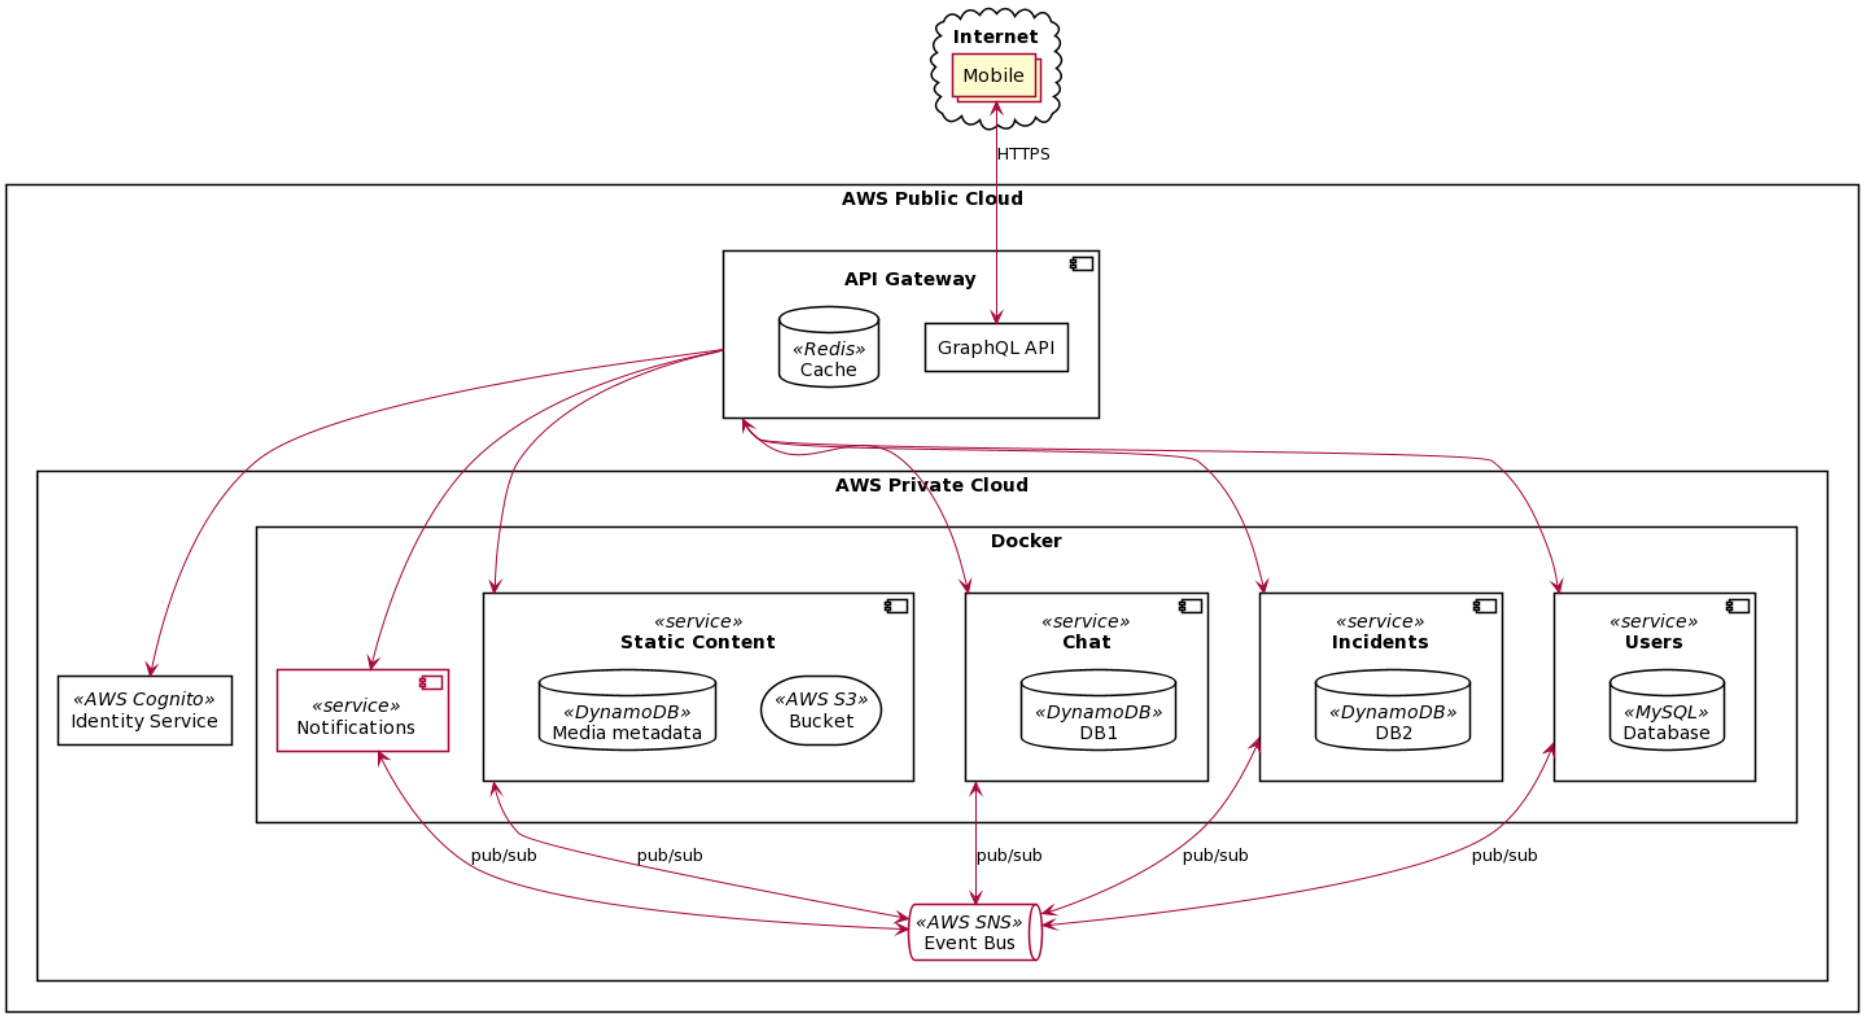
\includegraphics[scale=0.50]{figs/arquitetura.png}
	\label{f.diagrama-arquitetura}
	\legend{\small Fonte: Elaborada pelo autor.}
\end{figure}

\begin{figure}[htbp]
	\caption{\small Visão geral dos eventos assíncronos.}
	\centering
	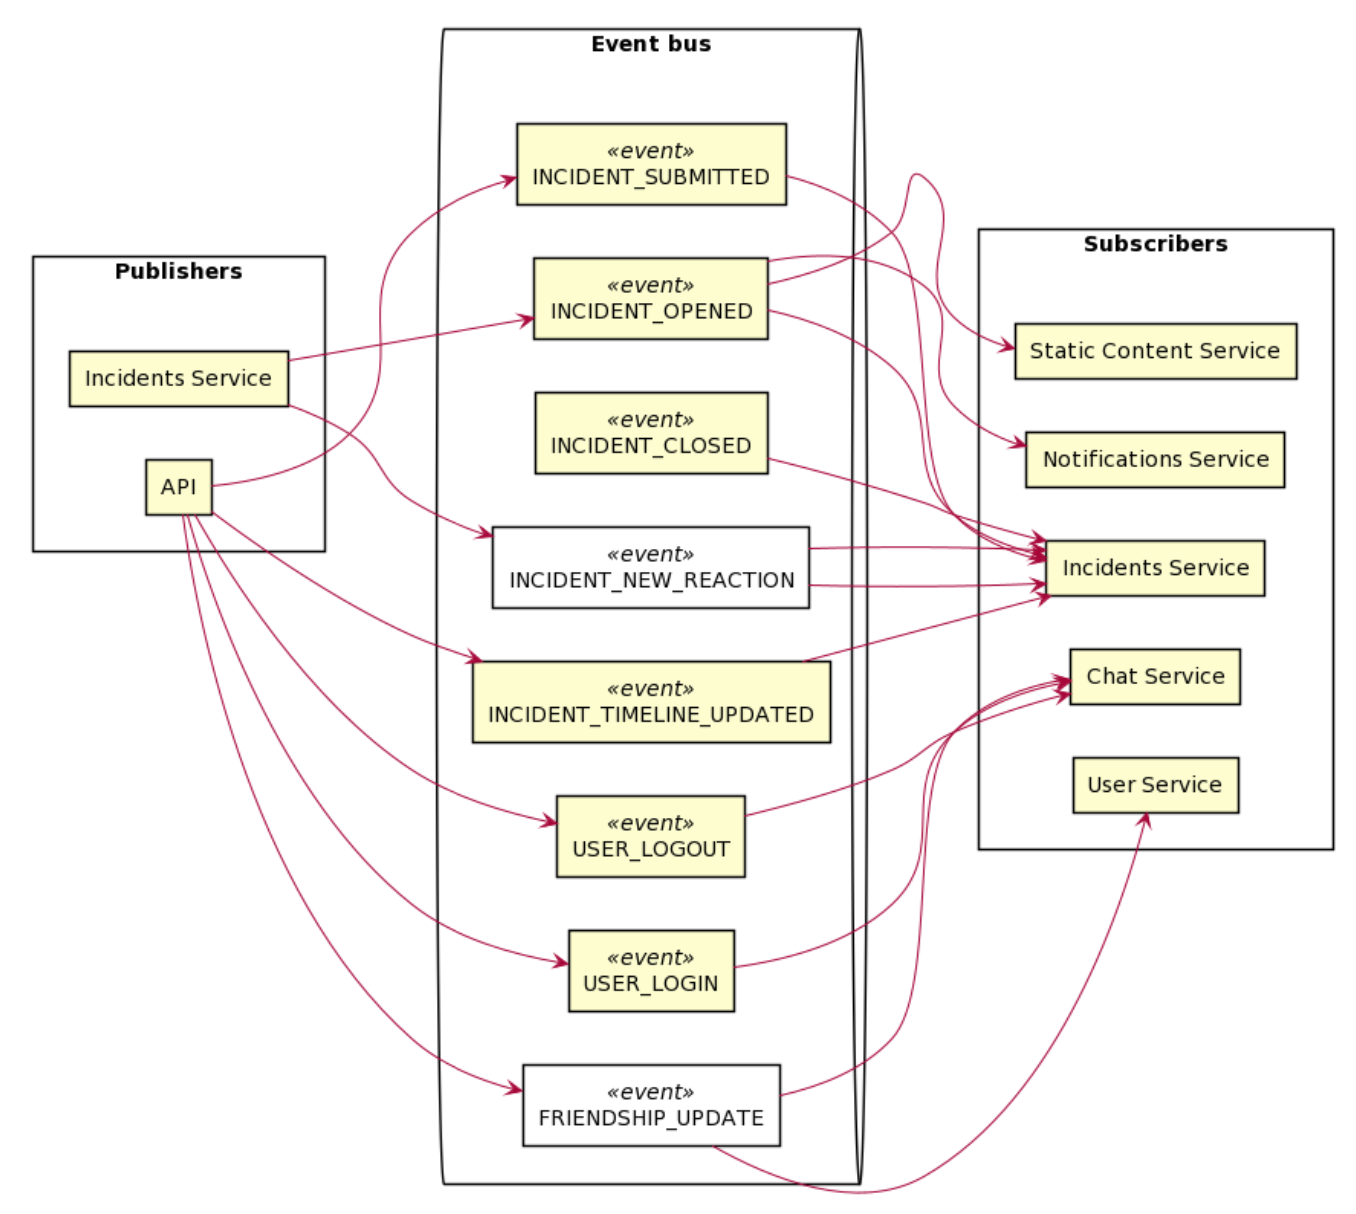
\includegraphics[scale=0.50]{figs/eventos.png}
	\label{f.diagrama-eventos}
	\legend{\small Fonte: Elaborada pelo autor.}
\end{figure}


Abaixo, a figura~\ref{f.diagrama-classes} ilustra as classes que representaram os dados persistidos no banco de dados.

\begin{figure}[htbp]
	\caption{\small Diagrama de classes.}
	\centering
	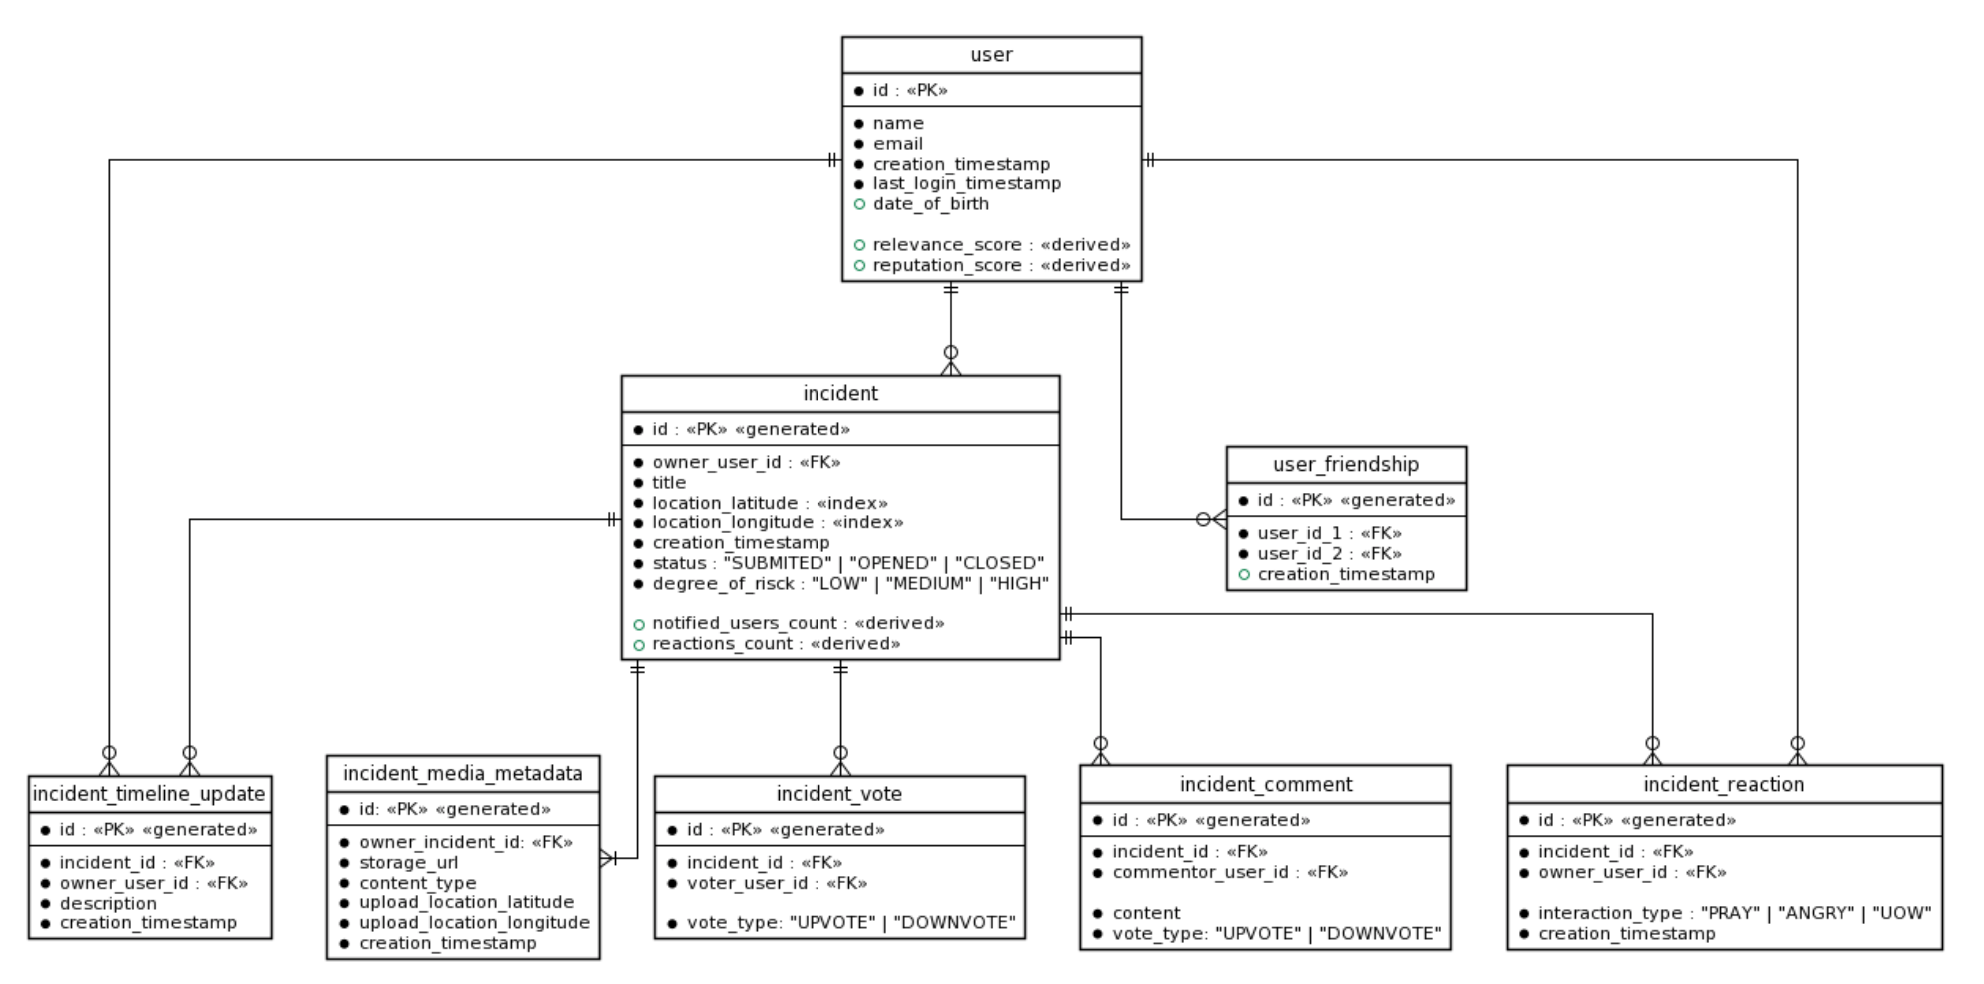
\includegraphics[scale=0.50]{figs/diagrama-de-classes.png}
	\label{f.diagrama-classes}
	\legend{\small Fonte: Elaborada pelo autor.}
\end{figure}


\chapter{Tecnologias pesquisadas e escolhidas}
\label{c.tecnologias}

% - Nesta seção cada equipe deverá pesquisar as alternativas de como cada um dos blocos propostos na seção anterior pode ser desenvolvido.
% - Dependendo da natureza de cada bloco, tecnologias podem ser microprocessadores, kits de desenvolvimento, linguagens de programação, protocolos de transmissão ou diferentes opções de algoritmos.
% - Após pesquisar a diferentes formas de desenvolver cada bloco o aluno deverá fazer uma escolha inicial, justificada, da tecnologia que pretende utilizar.
% - As tecnologias escolhidas devem ser descritas com mais detalhes. As tecnologias concorrentes podem ser apresentadas de maneira resumida, mas com detalhe suficiente para caracterizar sua funcionalidade, bem como seus aspectos positivos e negativos.

Para a implementaçãos, será adotada uma arquitetura baseada em microserviços e orientada à eventos. Os principais benefícios dessa escolha são: resiliência à falhas, baixo acoplamento, facilidade de escala, e facilidade para a coleta de dados.

O back-end será composto por aplicações conteinerizadas, que se comunicam de forma assíncrona via um sistema de mensageria. Aqueles serviços com maior demanda de entrada e saída (I/O-bound) serão escritos em NodeJS. E aqueles serviços com maior demanda de processamento computacional (CPU-bound) serão escritos em C\#.

Quanto à aplicação cliente, será adotado o React Native, um popular framework de código aberto mantido pelo Facebook que permite o desenvolvimento de aplicações móveis para múltiplas plataformas - iOS e Android - utilizando apenas JavaScript. 

Para suprir a infraestrutura computacional necessária, será utilizado serviços oferecidos por provedores de computação em nuvem, especialmente a Amazon Web Services (AWS). Entre as principais vantagens estão: alta disponibilidade de serviços, pagamento sob demanda, e agilidade no desenvolvimento.
\chapter{Procedimentos de validação do projeto}
\label{c.validacao}

% - Nesta seção devem ser indicados como os diversos módulos do projeto serão testados e validados individualmente e em conjunto.
% - Os testes gerais, que incluem o funcionamento do sistema do “ponto de vista do usuário”
% - Os testes do ambiente são usualmente denominados de “caixa preta”.
% - Os testes que permitem validar os módulos do projeto individualmente são usualmente denominados de “caixa branca”.
% - Nesta fase, a descrição dos testes poderá ser bem resumida, indicando principalmente os critérios de aceite do sistema e de cada um de seus módulos em termos do cumprimento de seus aspectos funcionais e de desempenho.

Cada módulo será testado de forma isolada, tendo em vista que eles estarão desacoplados por um sistema de mensageria.

Um entregável funcional chegará nas mãos do usuário final apenas após primeira entrega. Após o primeiro MVP, será coletado pontos de melhoria com alguns usuários selecionados. E após a finalização do projeto, a aplicação será monitadora, e os usuários serão questionados com pesquisas de satisfação.
\chapter{Riscos}
\label{c.riscos}

% - Nesta seção as equipes devem fazer uma análise dos problemas potenciais do projeto e do impacto desses problemas no seu sucesso ou fracasso (seguir a metodologia de engenharia de software).
% - Riscos típicos são:
%   - Aqueles relacionados à falta de componentes no mercado; 
%   - Atrasos na entrega de materiais;
%   - Falta de recursos materiais;
%   - Erro de estimativa da complexidade dos módulos;
%   - Escolha incorreta de implementação de algum módulo do sistema devido a tecnologia ser pouco conhecida.
% - Para os riscos que tiverem alto impacto na viabilidade do projeto, deverá ser previsto um plano de contingência.
% - Geralmente na forma de alteração da tecnologia de desenvolvimento de um módulo ou alteração de uma funcionalidade prevista.

O fato do sistema ser totalmente alimentado por usuários, e sobre um assunto sensível, faz com os pontos de atenção sejam muitos. O usuário pode, por exemplo, usar o aplicativo de forma não moderada, agindo como um "vigilante", "reporter criminal" ou até mesmo um "justiçeiro". 

O usuário pode não ser confiável. Ele pode fornecer alertas equivocados, difamatórios, racistas ou mentirosos, seja com intenção ou não. Nesses casos, as pessoas que tiverem sua imagem revelada, podem acabar recorrendo à justiça.

O usuário que mora em regiões mais perigosas pode ser alimentado constantemente por um sentimento de medo.

Questões de privacidade devem ser claras. O usuário precisa estar ciente que está compartilhando a sua localização o tempo todo, inclusive enquanto não está com o aplicativo aberto.

Questões filóficas também podem surgir entre os pensamentos dos usuários. Será que é melhor ser totalmente informado de todos os crimes e ficar possivelmente paranoico, ou ser totalmente ignorante deles mas viver em constante perigo?

\chapter{Cronograma do projeto}
\label{c.cronograma}

% - Descrever a data de início e a duração prevista para desenvolvimento de cada um dos módulos do projeto, assim como a pessoa responsável (no caso do projeto ser em equipe). Incluir as fases de documentação, desenvolvimento e testes.
% - As datas do cronograma do projeto devem ser compatíveis com as datas limites especificadas para as avaliações da disciplina de TCC.

É previsto que o desenvolvimento inicie a partir de 01/06/2021, e seja feito de forma iterativa, com a realização constante de testes unitários e de integração durante o processo de desenvolvimento.

A disponibilização do primeiro protótipo está prevista para 29/07/2021. Na seqência será coletado, portanto, os primeiros feedbacks e pontos de melhoria com os alguns usuários finais selecionados.


% TODO: SERIA BOM COLOCAR UMA FIGURA COM AS ETAPA
\chapter{Conclusão}
\label{c.conclusao}

% - A conclusão deve destacar os principais aspectos do projeto, os ganhos esperados, os principais desafios a serem enfrentados.
% - Deve-se dar uma avaliação geral da viabilidade do projeto.

O projeto visa atacar um problema sensível a todos: a segurança. O desafio, portanto, transcende as barreiras tecnológicas e e se tem suas raízes em questões culturais.

A nível de implementação o projeto é viável, tendo em vista que será totalmente baseado em nuvem.

As questões mais críticas são aquelas relacionadas ao ser humano. Mesmo com uma plataforma excepcional, e que permita a construção de um senso de comunidade, os valores das pessoas que o alimentam sempre estará em primeiro plano. Alguns países  com uma cultura de valorização do coletivismo pode usufruir melhor da plataforma, enquanto outros não.



% --------------------------------------------------------
% ELEMENTOS PÓS-TEXTUAIS
% --------------------------------------------------------

\postextual


% --------------------------------------------------------
% REFERÊNCIAS BIBLIOGRÁFICAS
% --------------------------------------------------------

\bibliography{chapters/referencias}


% --------------------------------------------------------
% GLOSSÁRIO
% --------------------------------------------------------

% Consulte o manual da classe abntex2 para orientações sobre o glossário.
%\glossary


% --------------------------------------------------------
% APÊNDICES
% --------------------------------------------------------

% Inicia os apêndices
%\begin{apendicesenv}
% Imprime uma página indicando o início dos apêndices
%\partapendices
% Criação do apêndice
%\end{apendicesenv}


% --------------------------------------------------------
% ÍNDICE REMISSIVO
% --------------------------------------------------------

%\printindex


% --------------------------------------------------------
% FINAL DO DOCUMENTO
% --------------------------------------------------------

\end{document}
